% portail-ajout-media.tex
\section{Ajouter des médias au profil}
En passant par la ligne de \textbf{stockage des média}, vous accéderez à une page spécifique montrant toutes les images que vous souhaitez stocker dans votre profil, hors du nuage étudié dans le chapitre idoine. 
Notez deux limitations :
\begin{itemize}
	\item l'espace maximum alloué est 100~Mo,
	\item chaque item ne peut pas dépasser la taille limite de 3~Mo
\end{itemize}
\begin{figure}
	\centering
	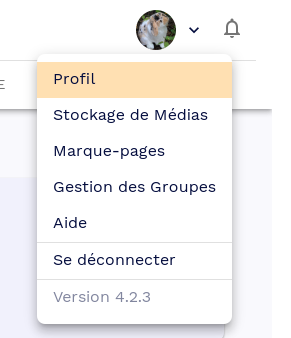
\includegraphics[width=0.3333\linewidth]{./Captures/menu.profil.png}
%	\caption{}
\end{figure}

\subsection{Ajouter un média}
Il existe deux méthodes pour ajouter un media à cet espace, le plus facile est d'ouvrir une fenêtre de l'explorateur de fichiers devant le navigateur, d'y sélectionner un ou plusieurs éléments, puis de les faire glisser sur la fenêtre du navigateur, les fichiers seront alors ajoutés à la liste des éléments présents.

L'autre méthode consiste à appuyer sur l'icône + à droite de la fenêtre, vers le haut.
\begin{figure}
	\centering
	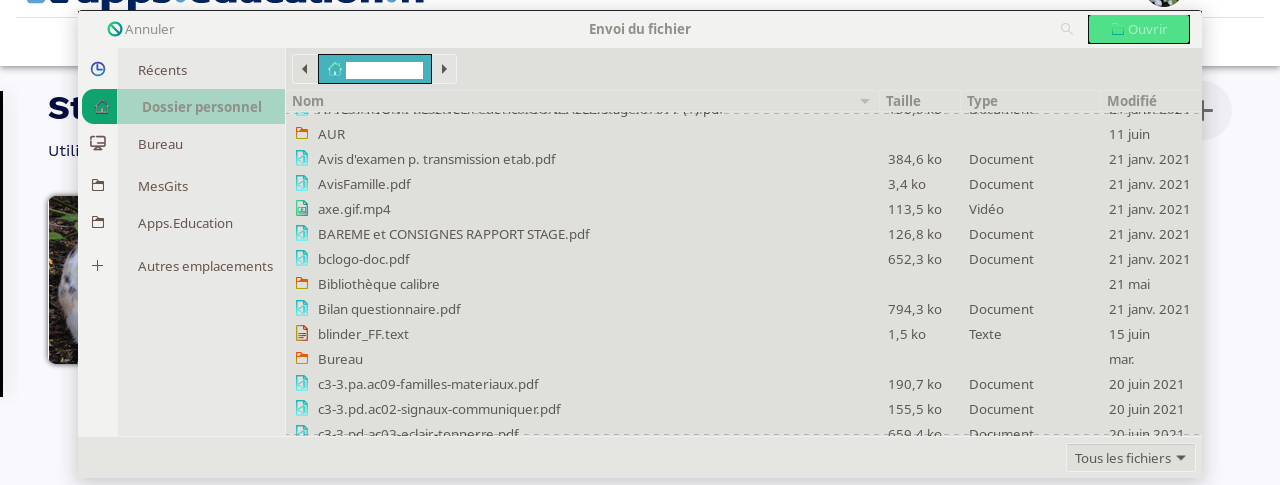
\includegraphics{./Captures/portail.stockage.medias.explorateur.png}
	\caption{L'appui sur ``+'' ouvre le navigateur local, ici en négatif car thème sombre originalement.}
\end{figure}
Une fenêtre de l'explorateur s'ouvrira, invitant l'utilisateur à choisir des éléments pour les y monter, comme le montre la capture plus haut
\begin{figure}
	\centering
	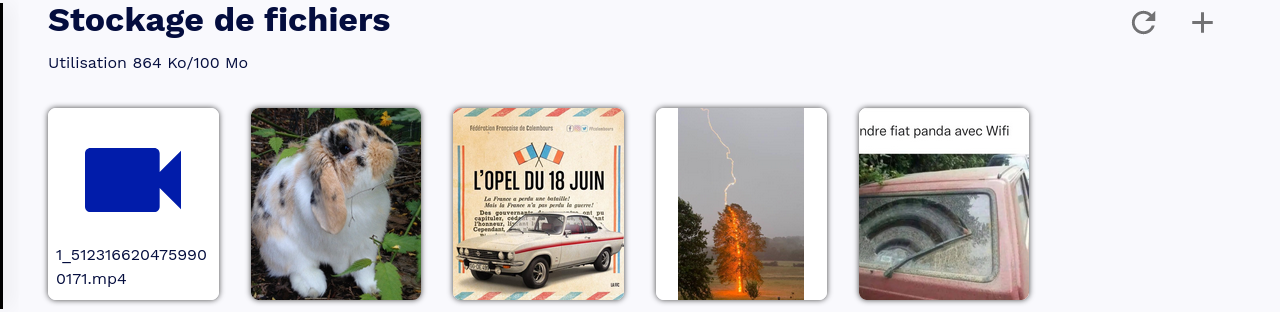
\includegraphics{./Captures/portail.stockage.medias.exemples.png}
	\caption{Affichage de quelques exemples déjà stockés sur mon profil.}
\end{figure}

\subsection{Gérer un média}
En sélectionnant un média, une mini-fenêtre de visualisation partielle (pour les images) ou de lecture (pour les vidéos) apparaît, elle se présente comme l'exemple qui suit.
\begin{figure}
	\centering
	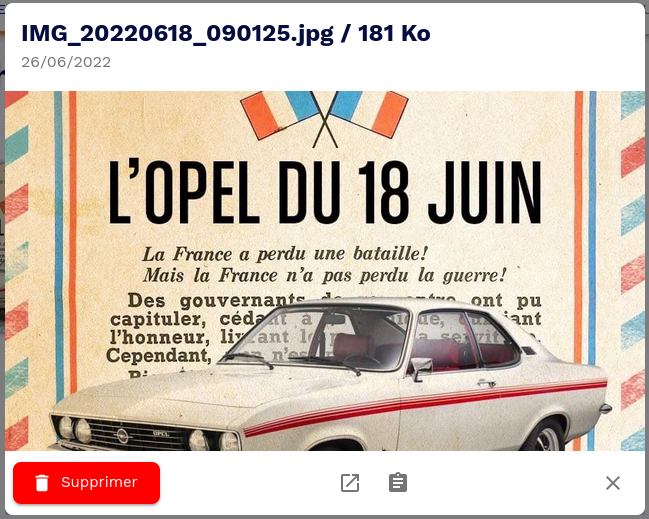
\includegraphics[width=0.500\linewidth]{./Captures/portail.stockage.medias.exemple.seul.png}
	\caption{Affichage d'un exemple de média stocké.}
\end{figure}
Vous aurez noté en haut le nom et la taille du document, quant à la partie basse elle présente une barre de gestion.
\begin{figure}
	\centering
	
\includegraphics[width=0.500\linewidth]{./Captures/portail.stockage.medias.barre.gestion.png}
	\caption{Les options de gestion d'une image stockée.}
\end{figure}
La barre de gestion des média affiche 4 options, de gauche à droite~:
\begin{itemize}
	\item un gros bouton rouge pour supprimer le média,
	\item un icône permettant d'afficher --sur mon navigateur cela déclenche le téléchargement-- du média dan sa totalité,
	\item un icône permettant de copier l'adresse de ce média,
	\item une croix pour fermer cette fenêtre.
\end{itemize}

\paragraph{Suppression d'un media.}
La suppression d'un média n'est pas directe et nécessite une double confirmation, en appuyant sur le gros bouton rouge, un compte à rebours de trois seconde s'enclenche pour valider cette suppression. 
À la fin du délais, si un second clic n'est pas venu attester le choix, la suppression n'est pas effective.
\begin{figure}
	\centering
	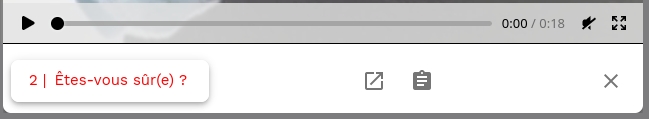
\includegraphics[width=0.500\linewidth]{./Captures/portail.stockage.medias.suppression.png}
	\caption{Suppression d'un média, êtes-vous sûr(e) ?}
\end{figure}
